\chapter{The PI3-Cluster Testbed}

\section{Installing an Operating System} \label{install_os}

To use the Raspberry Pi, an \gls{os} first needs to installed. \href{https://www.raspberrypi.org/downloads/raspbian/}{Raspbian Buster Lite} is the official \gls{os} for Raspberry Pi 3, and is used on the gateway and router. \href{https://www.freebsd.org/}{FreeBSD} is used on the hosts.

After downloading the \gls{os}, uncompress the file. The extracted file should be of type \lstinline{.img}, containing a preinstalled \gls{os} that now must be written to the SD card. To write the image file to the SD card, several tools exists that can be used, with some examples following:

\begin{itemize}
    \item Raspberry Pi Imager (official, cross-platform)
    \item balenaEtcher (cross-platform)
    \item \lstinline{dd} (Linux)
\end{itemize}

Once the image has been successfully written, simply put the SD card into the Raspberry Pi machine and boot it. On Raspbian Buster, the default user that comes preinstalled is called \lstinline{pi}, with the default password \lstinline{raspberry}. On FreeBSD, two users are installed by default; \lstinline{root} and \lstinline{freebsd}, with the password being the same as the username.


\section{Keyboard Layout} \label{keyboard_layout}

\subsubsection{Raspbian Buster}

To change keyboard layout with a graphical user guide, run \lstinline{dpkg-reconfigure keyboard-configuration}. The resulting changes is permanently added.

For most full-sized keyboards, the following options are what one may want; \lstinline{Generic 105-key PC (intl.) -> Norwegian -> Norwegian -> The default for the keyboard layout -> No compose key}.

\subsubsection{FreeBSD}

To change keyboard layout with a graphical user guide, run \lstinline{kbdmap}. To make the changes persist, add the resulting configuration to the \lstinline{/etc/rc.conf} file. For example, if Norwegian was selected, run \lstinline{echo 'keymap="no.kbd"' >> /etc/rc.conf}.


\section{Root Account} \label{root_account}

\subsubsection{Raspbian Buster}

Once logged in with user \lstinline{pi}, create a root user with \lstinline{sudo passwd root}. Enter a chosen password. A root user has now been created. To use it, log out with \lstinline{logout} or simply reboot, and then log in as \lstinline{root}.

To delete the \lstinline{pi} user, issue the command \lstinline{deluser --remove-home pi} while logged in as \lstinline{root}.

\subsubsection{FreeBSD}

FreeBSD already comes preinstalled with two user accounts; \lstinline{root} and \lstinline{freebsd}. To delete the \lstinline{freebsd} user, log in as \lstinline{root} and run \lstinline{rmuser freebsd}.


\section{Updating the System} \label{update_system}

\subsubsection{Raspbian Buster}

\textbf{Note:} \textit{If the current system is using a custom kernel, upgrading the system will also upgrade the kernel, thus overwriting the custom kernel. One can omit the \lstinline{upgrade} part if that is not desired.}

To update the system, run \lstinline{apt update && apt upgrade}. If an error about \lstinline{release file not valid yet} appears, the system's clock needs to be fixed. This can easily be done with the \lstinline{date} tool; \lstinline{date -s "15 Feb 2020 12:00"}.

\subsubsection{FreeBSD}

To update the system, run the following:

\begin{minted}{bash}
# Update FreeBSD system
freebsd-update fetch && freebsd-update install

# Update FreeBSD packages
pkg upgrade
\end{minted}


\section{Enable SSH} \label{enable_ssh}

\subsubsection{Raspbian Buster}

To enable SSH access, simply run \lstinline{systemctl enable ssh}. To allow SSH root login, the line \lstinline{PermitRootLogin yes} must be added to the file \lstinline{/etc/ssh/sshd_config}, which can conveniently be done with \lstinline{echo 'PermitRootLogin yes' >> /etc/ssh/sshd_config}. Then start SSH service with \lstinline{systemctl start ssh} or just reboot.

\subsubsection{FreeBSD}

SSH on FreeBSD is installed and enabled by default as seen by \lstinline{sshd_enable="YES"} in the file \lstinline{/etc/rc.conf}. However, root login must be explicitly allowed; \lstinline{echo 'PermitRootLogin yes' >> /etc/ssh/sshd_config}. Reboot to apply the changes.

\textit{Note}: SSH access on FreeBSD can sometimes experience a long delay when establishing a connection. If this is the case, DNS lookup can be disabled with \lstinline{echo 'UseDNS no' >> /etc/ssh/sshd_config}.


\section{Change Hostname} \label{change_hostname}

\subsubsection{Raspbian Buster}

There are two files that needs to be edited in order to change hostname. First, the \lstinline{/etc/hostname} file, which only contains the current hostname. Simply change whatever is in it to what you want, say \lstinline{new_hostname}. Second, the file \lstinline{/etc/hosts} needs one line changed. Edit the line containg \lstinline{127.0.1.1} so that it looks as follows:

\begin{minted}{bash}
127.0.1.1       new_hostname
\end{minted}

A reboot will apply the changes.

\subsubsection{FreeBSD}

Only one file need to be changed. Open up the \lstinline{/etc/rc.conf} file, and replace the \lstinline{hostname} entry with the desired hostname. Reboot to apply the changes.


\section{Time Synchronization} \label{time_sync}

First, set up a common timezone on all machines. On Raspbian Buster, run \lstinline{timedatectl set-timezone CET}. On FreeBSD, run \lstinline{tzsetup CET}.

\subsubsection{NTP Server on Raspbian Buster}

Install \lstinline{ntp} with \lstinline{apt install ntp}. Then check if any \gls{ntp} peers are connected with \lstinline{ntpq -p}. If not, consider replacing the default pools or servers in \lstinline{/etc/ntp.conf} with another, such as \lstinline{server ntp.uio.no} followed up by \lstinline{systemctl restart ntp}.

\subsubsection{NTP Client on Raspbian Buster}

To automatically query for time from the \gls{ntp} server, the Raspbian Buster \gls{os} already comes with a lightweight daemon called \lstinline{systemd-timesyncd} that allows for synchronizing the system clock across the network. However, TEACUP prefers to use \lstinline{ntp} instead, and so \lstinline{ntp} will be used.

Install \lstinline{ntp} with \lstinline{apt install ntp}. To specify which server to get the time from, prepare to edit the \lstinline{/etc/ntp.conf} file. Comment out the default pools, and add the entry \lstinline{server 10.0.1.254 iburst} which refers to the gateway.

Next, disable the \lstinline{systemd-timesyncd} with \lstinline{timedatectl set-ntp false} as we are using \lstinline{ntp} directly to update the time. Finally, either restart the service with \lstinline{systemctl restart ntp} or reboot. Wait a bit, and verify time synchronization with either \lstinline{ntpq -p} or simply \lstinline{date}.

\subsubsection{NTP Client on FreeBSD}

FreeBSD comes preinstalled with \lstinline{ntp}. To enable it on boot, run the following:

\begin{minted}{bash}
# Enable NTP on FreeBSD
echo 'ntpd_enable=YES' >> /etc/rc.conf
echo 'ntpd_sync_on_start=YES' >> /etc/rc.conf
\end{minted}

To specify which server to get the time from, prepare to edit the \lstinline{/etc/ntp.conf} file. Comment out any default pool or server entries, and add the new entry \lstinline{server 10.0.1.254 iburst} to it, which refers to the gateway. Reboot and verify time synchronization with \lstinline{date}.























% \chapter{The PI4-Cluster Testbed}

% \section{Setting Up Dual Boot}

% First install Ubuntu. When asked for partitioning the disk, choose \lstinline{manual}, select the disk and confirm creating a new empty partition with \lstinline{yes}. Select the newly created empty partition followed by \lstinline{create a new partition} and set a size for it. The type should be of \lstinline{primary}, location at \lstinline{beginning} and mounting point \lstinline{root}. Finish off with \lstinline{done setting up the partition} followed by \lstinline{finish partitioning and write changes to disk}.

% \begin{figure}[H]
%     \centering
%     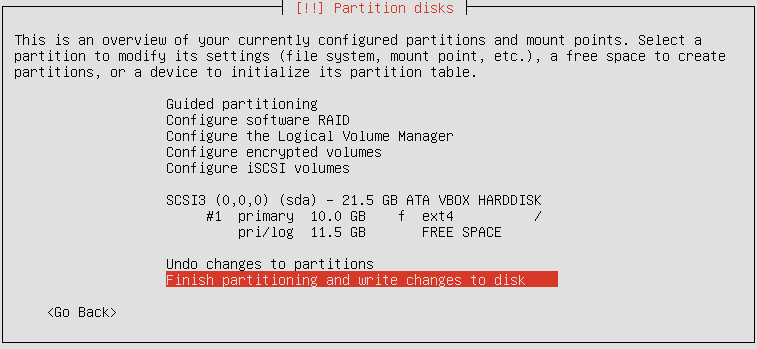
\includegraphics[width=0.75\linewidth]{ubuntu_partition}
%     \captionsetup{width=0.75\linewidth}
%     \caption{The partition editor for Ubuntu.}
%     \label{fig:ubuntu_partition}
% \end{figure}

% Next, install FreeBSD. When asked for partitioning the disk, choose \lstinline{auto (UFS)} followed by \lstinline{partition}. Set a size, hit \lstinline{ok} and \lstinline{finish}.

% \begin{figure}[H]
%     \centering
%     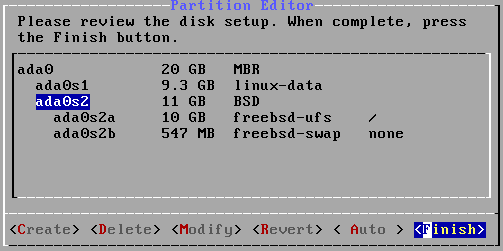
\includegraphics[width=0.75\linewidth]{freebsd_partition}
%     \captionsetup{width=0.75\linewidth}
%     \caption{The partition editor for FreeBSD.}
%     \label{fig:freebsd_partition}
% \end{figure}

% After installing both systems, only Ubuntu is presented in the \gls{grub}. To add FreeBSD as an option, run \lstinline{sudo nano /etc/grub.d/40_custom} in Ubuntu, and add the following entry:

% \begin{minted}{bash}
% menuentry "FreeBSD" {
%     insmod ufs2
%     set root=(hd0,2)
%     kfreebsd /boot/loader
% }
% \end{minted}

% Then update \gls{grub} with \lstinline{sudo update-grub}. The FreeBSD option should now be available when rebooting. If the bootloader won't display, hold the \lstinline{RIGHT SHIFT} key upon booting.

% To enable a one-time reboot into FreeBSD from Ubuntu, run the command \lstinline{grub-editenv /boot/grub/grubenv set next_entry="FreeBSD"} and reboot with \lstinline{sudo reboot}.





% \section{Compiling Mainline Kernel 5.5 for Raspberry Pi 4}


% \section{Patching web10g on Mainline Kernel 5.5}